\documentclass[twoside]{book}

% Packages required by doxygen
\usepackage{fixltx2e}
\usepackage{calc}
\usepackage{doxygen}
\usepackage[export]{adjustbox} % also loads graphicx
\usepackage{graphicx}
\usepackage[utf8]{inputenc}
\usepackage{makeidx}
\usepackage{multicol}
\usepackage{multirow}
\PassOptionsToPackage{warn}{textcomp}
\usepackage{textcomp}
\usepackage[nointegrals]{wasysym}
\usepackage[table]{xcolor}

% Font selection
\usepackage[T1]{fontenc}
\usepackage[scaled=.90]{helvet}
\usepackage{courier}
\usepackage{amssymb}
\usepackage{sectsty}
\renewcommand{\familydefault}{\sfdefault}
\allsectionsfont{%
  \fontseries{bc}\selectfont%
  \color{darkgray}%
}
\renewcommand{\DoxyLabelFont}{%
  \fontseries{bc}\selectfont%
  \color{darkgray}%
}
\newcommand{\+}{\discretionary{\mbox{\scriptsize$\hookleftarrow$}}{}{}}

% Page & text layout
\usepackage{geometry}
\geometry{%
  a4paper,%
  top=2.5cm,%
  bottom=2.5cm,%
  left=2.5cm,%
  right=2.5cm%
}
\tolerance=750
\hfuzz=15pt
\hbadness=750
\setlength{\emergencystretch}{15pt}
\setlength{\parindent}{0cm}
\setlength{\parskip}{0.2cm}
\makeatletter
\renewcommand{\paragraph}{%
  \@startsection{paragraph}{4}{0ex}{-1.0ex}{1.0ex}{%
    \normalfont\normalsize\bfseries\SS@parafont%
  }%
}
\renewcommand{\subparagraph}{%
  \@startsection{subparagraph}{5}{0ex}{-1.0ex}{1.0ex}{%
    \normalfont\normalsize\bfseries\SS@subparafont%
  }%
}
\makeatother

% Headers & footers
\usepackage{fancyhdr}
\pagestyle{fancyplain}
\fancyhead[LE]{\fancyplain{}{\bfseries\thepage}}
\fancyhead[CE]{\fancyplain{}{}}
\fancyhead[RE]{\fancyplain{}{\bfseries\leftmark}}
\fancyhead[LO]{\fancyplain{}{\bfseries\rightmark}}
\fancyhead[CO]{\fancyplain{}{}}
\fancyhead[RO]{\fancyplain{}{\bfseries\thepage}}
\fancyfoot[LE]{\fancyplain{}{}}
\fancyfoot[CE]{\fancyplain{}{}}
\fancyfoot[RE]{\fancyplain{}{\bfseries\scriptsize Generated on Mon Jun 6 2016 09\+:56\+:59 for Oscilloscope by Doxygen }}
\fancyfoot[LO]{\fancyplain{}{\bfseries\scriptsize Generated on Mon Jun 6 2016 09\+:56\+:59 for Oscilloscope by Doxygen }}
\fancyfoot[CO]{\fancyplain{}{}}
\fancyfoot[RO]{\fancyplain{}{}}
\renewcommand{\footrulewidth}{0.4pt}
\renewcommand{\chaptermark}[1]{%
  \markboth{#1}{}%
}
\renewcommand{\sectionmark}[1]{%
  \markright{\thesection\ #1}%
}

% Indices & bibliography
\usepackage{natbib}
\usepackage[titles]{tocloft}
\setcounter{tocdepth}{3}
\setcounter{secnumdepth}{5}
\makeindex

% Hyperlinks (required, but should be loaded last)
\usepackage{ifpdf}
\ifpdf
  \usepackage[pdftex,pagebackref=true]{hyperref}
\else
  \usepackage[ps2pdf,pagebackref=true]{hyperref}
\fi
\hypersetup{%
  colorlinks=true,%
  linkcolor=blue,%
  citecolor=blue,%
  unicode%
}

% Custom commands
\newcommand{\clearemptydoublepage}{%
  \newpage{\pagestyle{empty}\cleardoublepage}%
}


%===== C O N T E N T S =====

\begin{document}

% Titlepage & ToC
\hypersetup{pageanchor=false,
             bookmarks=true,
             bookmarksnumbered=true,
             pdfencoding=unicode
            }
\pagenumbering{roman}
\begin{titlepage}
\vspace*{7cm}
\begin{center}%
{\Large Oscilloscope }\\
\vspace*{1cm}
{\large Generated by Doxygen 1.8.9.1}\\
\vspace*{0.5cm}
{\small Mon Jun 6 2016 09:56:59}\\
\end{center}
\end{titlepage}
\clearemptydoublepage
\tableofcontents
\clearemptydoublepage
\pagenumbering{arabic}
\hypersetup{pageanchor=true}

%--- Begin generated contents ---
\chapter{File Index}
\section{File List}
Here is a list of all documented files with brief descriptions\+:\begin{DoxyCompactList}
\item\contentsline{section}{Oscilloscope/src/\hyperlink{LCDgraphic_8c}{L\+C\+Dgraphic.\+c} \\*Library with functions for graphical L\+C\+D based on K\+S0108 }{\pageref{LCDgraphic_8c}}{}
\item\contentsline{section}{Oscilloscope/src/\hyperlink{LCDgraphic_8h}{L\+C\+Dgraphic.\+h} \\*Library with utility functions for graphical L\+C\+D based on K\+S0108 }{\pageref{LCDgraphic_8h}}{}
\item\contentsline{section}{Oscilloscope/src/\hyperlink{main_8c}{main.\+c} \\*Oscilloscope based on P\+I\+C18\+F4550 and 128x64 Graphic L\+C\+D }{\pageref{main_8c}}{}
\end{DoxyCompactList}

\chapter{File Documentation}
\hypertarget{LCDgraphic_8c}{}\section{Oscilloscope/src/\+L\+C\+Dgraphic.c File Reference}
\label{LCDgraphic_8c}\index{Oscilloscope/src/\+L\+C\+Dgraphic.\+c@{Oscilloscope/src/\+L\+C\+Dgraphic.\+c}}


Library with functions for graphical L\+C\+D based on K\+S0108.  


{\ttfamily \#include \char`\"{}L\+C\+Dgraphic.\+h\char`\"{}}\\*
{\ttfamily \#include $<$xc.\+h$>$}\\*
{\ttfamily \#include $<$string.\+h$>$}\\*
Include dependency graph for L\+C\+Dgraphic.\+c\+:\nopagebreak
\begin{figure}[H]
\begin{center}
\leavevmode
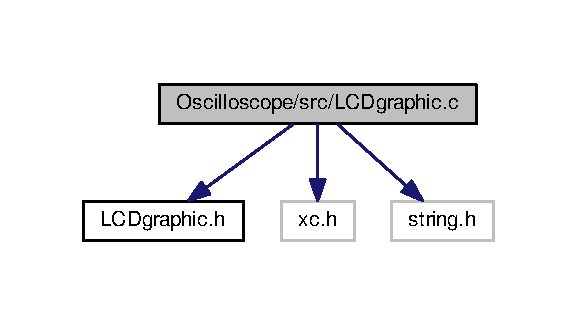
\includegraphics[width=277pt]{LCDgraphic_8c__incl}
\end{center}
\end{figure}
\subsection*{Macros}
\begin{DoxyCompactItemize}
\item 
\hypertarget{LCDgraphic_8c_a2f51b05c046cc617b8cceea73ef2aa41}{}\#define {\bfseries L\+C\+D\+\_\+\+T\+R\+I\+S}~T\+R\+I\+S\+D\label{LCDgraphic_8c_a2f51b05c046cc617b8cceea73ef2aa41}

\item 
\hypertarget{LCDgraphic_8c_a25e9d818788f36ed74d7c4579f87f2a6}{}\#define {\bfseries L\+C\+D\+\_\+\+D\+A\+T\+A}~P\+O\+R\+T\+D\label{LCDgraphic_8c_a25e9d818788f36ed74d7c4579f87f2a6}

\item 
\hypertarget{LCDgraphic_8c_a22e6626f2c98ed902f8ded47f6438c05}{}\#define {\bfseries E\+N}~L\+A\+T\+Cbits.\+L\+A\+T\+C0\label{LCDgraphic_8c_a22e6626f2c98ed902f8ded47f6438c05}

\item 
\hypertarget{LCDgraphic_8c_afc4ded33ac0ca43defcce639e965748a}{}\#define {\bfseries R\+W}~L\+A\+T\+Cbits.\+L\+A\+T\+C1\label{LCDgraphic_8c_afc4ded33ac0ca43defcce639e965748a}

\item 
\hypertarget{LCDgraphic_8c_af8903d8eea3868940c60af887473b152}{}\#define {\bfseries R\+S}~L\+A\+T\+Cbits.\+L\+A\+T\+C2\label{LCDgraphic_8c_af8903d8eea3868940c60af887473b152}

\item 
\hypertarget{LCDgraphic_8c_afc3c191d4a580107456963e1286b3d42}{}\#define {\bfseries C\+S1}~L\+A\+T\+Ebits.\+L\+A\+T\+E0\label{LCDgraphic_8c_afc3c191d4a580107456963e1286b3d42}

\item 
\hypertarget{LCDgraphic_8c_a3e759404ee1066f529adc98fab60ff21}{}\#define {\bfseries C\+S2}~L\+A\+T\+Ebits.\+L\+A\+T\+E1\label{LCDgraphic_8c_a3e759404ee1066f529adc98fab60ff21}

\item 
\hypertarget{LCDgraphic_8c_ac030a53d0878ffe6e5785fad3ea8ed50}{}\#define {\bfseries R\+E\+S\+E\+T\+\_\+\+L\+C\+D}~L\+A\+T\+Cbits.\+L\+A\+T\+C6\label{LCDgraphic_8c_ac030a53d0878ffe6e5785fad3ea8ed50}

\item 
\hypertarget{LCDgraphic_8c_a024148e99a7143db044a48216664d03d}{}\#define {\bfseries \+\_\+\+X\+T\+A\+L\+\_\+\+F\+R\+E\+Q}~40000000\label{LCDgraphic_8c_a024148e99a7143db044a48216664d03d}

\end{DoxyCompactItemize}
\subsection*{Functions}
\begin{DoxyCompactItemize}
\item 
void \hyperlink{LCDgraphic_8c_a11d5b0d5ef5f8579a4e8d8b078075ec3}{\+\_\+lcd\+\_\+enable} (void)
\begin{DoxyCompactList}\small\item\em Sends the enable pulse. \end{DoxyCompactList}\item 
void \hyperlink{LCDgraphic_8c_a77153afe052be2c883ce0e9c50eaf63d}{L\+C\+Dinit} ()
\begin{DoxyCompactList}\small\item\em Initializes the L\+C\+D. \end{DoxyCompactList}\item 
unsigned char \hyperlink{LCDgraphic_8c_a26ad6217905851ea5c3110a290b6fdb3}{\+\_\+lcd\+\_\+status} (void)
\begin{DoxyCompactList}\small\item\em Reads the status of the L\+C\+D. \end{DoxyCompactList}\item 
void \hyperlink{LCDgraphic_8c_a33c82f86c90f14e8e52f13de0228830d}{L\+C\+Dcmd} (unsigned char data)
\begin{DoxyCompactList}\small\item\em Sends a command to the L\+C\+D. \end{DoxyCompactList}\item 
void \hyperlink{LCDgraphic_8c_a9e0d454df8127abcf7ee2e962b6dd18e}{L\+C\+Dreset} (void)
\begin{DoxyCompactList}\small\item\em Resets the L\+C\+D. \end{DoxyCompactList}\item 
void \hyperlink{LCDgraphic_8c_a414751e33fa233791c30874c6737660d}{\+\_\+lcd\+\_\+waitbusy} (void)
\begin{DoxyCompactList}\small\item\em Waits until the L\+C\+D can accept new commands. \end{DoxyCompactList}\item 
char \hyperlink{LCDgraphic_8c_a84265c7d35e130b40e65accc9196db7f}{L\+C\+Dpage} (unsigned char side, unsigned char page)
\begin{DoxyCompactList}\small\item\em Selects a page from one of the two sides. \end{DoxyCompactList}\item 
void \hyperlink{LCDgraphic_8c_a40db310206fc27ed314f3b955754ee56}{L\+C\+Don} (unsigned char on)
\begin{DoxyCompactList}\small\item\em Turns O\+N/\+O\+F\+F the L\+C\+D. \end{DoxyCompactList}\item 
char \hyperlink{LCDgraphic_8c_ac8fd49b1549fc88864cab720cffe7c26}{L\+C\+Dy} (unsigned char side, unsigned char value)
\begin{DoxyCompactList}\small\item\em Specifies a column in the selected page. \end{DoxyCompactList}\item 
void \hyperlink{LCDgraphic_8c_ac55e028c6bfe194ffb28f3e2b8b259b2}{emptycolumn} (void)
\begin{DoxyCompactList}\small\item\em Writes space between adjacent letters. \end{DoxyCompactList}\item 
char \hyperlink{LCDgraphic_8c_a86bbf9d181141b4501339701328da802}{L\+C\+Dchar} (unsigned char c, unsigned char position)
\begin{DoxyCompactList}\small\item\em Writes an A\+S\+C\+I\+I character to the display. \end{DoxyCompactList}\item 
void \hyperlink{LCDgraphic_8c_a28e765a7041cb850f82f1e7b36ef4898}{L\+C\+Dclear} (void)
\begin{DoxyCompactList}\small\item\em Clears all the data in the display. \end{DoxyCompactList}\item 
char \hyperlink{LCDgraphic_8c_ae1800a1561ae35e4275a2653532dcb31}{L\+C\+Dstring} (char p, const char $\ast$buffer)
\begin{DoxyCompactList}\small\item\em Writes a string to the L\+C\+D. \end{DoxyCompactList}\item 
char \hyperlink{LCDgraphic_8c_a1e45984915a2f1966a97fb3bd653bd7d}{lcdplotpixel2} (char rx, char ry, int blank)
\begin{DoxyCompactList}\small\item\em Turns on or off pixels accordingly to blank parameter. \end{DoxyCompactList}\item 
void \hyperlink{LCDgraphic_8c_acbbed37c26fb794eb90f33c9a3613649}{xyaxis} ()
\begin{DoxyCompactList}\small\item\em Draws the xy axis grid. \end{DoxyCompactList}\item 
char \hyperlink{LCDgraphic_8c_a2308346cd773ff7850bac3858143d261}{L\+C\+D\+Startline} (unsigned char side, unsigned char value)
\begin{DoxyCompactList}\small\item\em Set L\+C\+D start line. \end{DoxyCompactList}\item 
unsigned char \hyperlink{LCDgraphic_8c_a6c9fd9c7e01c9248bd553add98897244}{L\+C\+Dread} ()
\begin{DoxyCompactList}\small\item\em Returns the data written at the previously set page and column. \end{DoxyCompactList}\item 
void \hyperlink{LCDgraphic_8c_ab25dd805ae6efe3ebd124f40d92421ec}{write\+\_\+image} (const char $\ast$image, char top\+\_\+to\+\_\+bottom)
\begin{DoxyCompactList}\small\item\em Writes an image to the screen. \end{DoxyCompactList}\end{DoxyCompactItemize}
\subsection*{Variables}
\begin{DoxyCompactItemize}
\item 
\hypertarget{LCDgraphic_8c_ad33bb4de3af63117d1de6cfd984fa375}{}char const {\bfseries pic} \mbox{[}$\,$\mbox{]}\mbox{[}5\mbox{]}\label{LCDgraphic_8c_ad33bb4de3af63117d1de6cfd984fa375}

\end{DoxyCompactItemize}


\subsection{Detailed Description}
Library with functions for graphical L\+C\+D based on K\+S0108. 

\begin{DoxyAuthor}{Author}
Davide Lucchi 
\end{DoxyAuthor}
\begin{DoxyVersion}{Version}
1.\+0 
\end{DoxyVersion}
\begin{DoxySince}{Since}
1.\+0 
\end{DoxySince}


\subsection{Function Documentation}
\hypertarget{LCDgraphic_8c_a11d5b0d5ef5f8579a4e8d8b078075ec3}{}\index{L\+C\+Dgraphic.\+c@{L\+C\+Dgraphic.\+c}!\+\_\+lcd\+\_\+enable@{\+\_\+lcd\+\_\+enable}}
\index{\+\_\+lcd\+\_\+enable@{\+\_\+lcd\+\_\+enable}!L\+C\+Dgraphic.\+c@{L\+C\+Dgraphic.\+c}}
\subsubsection[{\+\_\+lcd\+\_\+enable}]{\setlength{\rightskip}{0pt plus 5cm}void \+\_\+lcd\+\_\+enable (
\begin{DoxyParamCaption}
\item[{void}]{}
\end{DoxyParamCaption}
)}\label{LCDgraphic_8c_a11d5b0d5ef5f8579a4e8d8b078075ec3}


Sends the enable pulse. 

It sends an enable pulse to the L\+C\+D. On the rising edge the L\+C\+D puts/reads the data to/from the bus accordingly to the read/write bit value

\begin{DoxyReturn}{Returns}
nothing
\end{DoxyReturn}
\begin{DoxyAuthor}{Author}
Davide Lucchi 
\end{DoxyAuthor}
\begin{DoxyVersion}{Version}
1.\+0 
\end{DoxyVersion}
\begin{DoxySince}{Since}
1.\+0 
\end{DoxySince}
\hypertarget{LCDgraphic_8c_a26ad6217905851ea5c3110a290b6fdb3}{}\index{L\+C\+Dgraphic.\+c@{L\+C\+Dgraphic.\+c}!\+\_\+lcd\+\_\+status@{\+\_\+lcd\+\_\+status}}
\index{\+\_\+lcd\+\_\+status@{\+\_\+lcd\+\_\+status}!L\+C\+Dgraphic.\+c@{L\+C\+Dgraphic.\+c}}
\subsubsection[{\+\_\+lcd\+\_\+status}]{\setlength{\rightskip}{0pt plus 5cm}unsigned char \+\_\+lcd\+\_\+status (
\begin{DoxyParamCaption}
\item[{void}]{}
\end{DoxyParamCaption}
)}\label{LCDgraphic_8c_a26ad6217905851ea5c3110a290b6fdb3}


Reads the status of the L\+C\+D. 

It sends a request to the L\+C\+D to make it put its status on the data bus. The M\+S\+B of the status contains the B\+U\+S\+Y flag, the 3rd M\+S\+B the display O\+N/\+O\+F\+F flag and the 4th M\+S\+B the R\+E\+S\+E\+T flag.

\begin{DoxyReturn}{Returns}
The L\+C\+D status
\end{DoxyReturn}
\begin{DoxyAuthor}{Author}
Davide Lucchi 
\end{DoxyAuthor}
\begin{DoxyVersion}{Version}
1.\+0 
\end{DoxyVersion}
\begin{DoxySince}{Since}
1.\+0 
\end{DoxySince}
\hypertarget{LCDgraphic_8c_a414751e33fa233791c30874c6737660d}{}\index{L\+C\+Dgraphic.\+c@{L\+C\+Dgraphic.\+c}!\+\_\+lcd\+\_\+waitbusy@{\+\_\+lcd\+\_\+waitbusy}}
\index{\+\_\+lcd\+\_\+waitbusy@{\+\_\+lcd\+\_\+waitbusy}!L\+C\+Dgraphic.\+c@{L\+C\+Dgraphic.\+c}}
\subsubsection[{\+\_\+lcd\+\_\+waitbusy}]{\setlength{\rightskip}{0pt plus 5cm}void \+\_\+lcd\+\_\+waitbusy (
\begin{DoxyParamCaption}
\item[{void}]{}
\end{DoxyParamCaption}
)}\label{LCDgraphic_8c_a414751e33fa233791c30874c6737660d}


Waits until the L\+C\+D can accept new commands. 

It keeps requesting the L\+C\+D status until the B\+U\+S\+Y and R\+E\+S\+E\+T flags are cleared.

\begin{DoxyReturn}{Returns}
nothing
\end{DoxyReturn}
\begin{DoxyAuthor}{Author}
Davide Lucchi 
\end{DoxyAuthor}
\begin{DoxyVersion}{Version}
1.\+0 
\end{DoxyVersion}
\begin{DoxySince}{Since}
1.\+0 
\end{DoxySince}
\hypertarget{LCDgraphic_8c_ac55e028c6bfe194ffb28f3e2b8b259b2}{}\index{L\+C\+Dgraphic.\+c@{L\+C\+Dgraphic.\+c}!emptycolumn@{emptycolumn}}
\index{emptycolumn@{emptycolumn}!L\+C\+Dgraphic.\+c@{L\+C\+Dgraphic.\+c}}
\subsubsection[{emptycolumn}]{\setlength{\rightskip}{0pt plus 5cm}void emptycolumn (
\begin{DoxyParamCaption}
\item[{void}]{}
\end{DoxyParamCaption}
)}\label{LCDgraphic_8c_ac55e028c6bfe194ffb28f3e2b8b259b2}


Writes space between adjacent letters. 

Writes an empty column after the last written letter

\begin{DoxyReturn}{Returns}
nothing
\end{DoxyReturn}
\begin{DoxyAuthor}{Author}
Davide Lucchi 
\end{DoxyAuthor}
\begin{DoxyVersion}{Version}
1.\+0 
\end{DoxyVersion}
\begin{DoxySince}{Since}
1.\+0 
\end{DoxySince}
\hypertarget{LCDgraphic_8c_a86bbf9d181141b4501339701328da802}{}\index{L\+C\+Dgraphic.\+c@{L\+C\+Dgraphic.\+c}!L\+C\+Dchar@{L\+C\+Dchar}}
\index{L\+C\+Dchar@{L\+C\+Dchar}!L\+C\+Dgraphic.\+c@{L\+C\+Dgraphic.\+c}}
\subsubsection[{L\+C\+Dchar}]{\setlength{\rightskip}{0pt plus 5cm}char L\+C\+Dchar (
\begin{DoxyParamCaption}
\item[{unsigned char}]{c, }
\item[{unsigned char}]{position}
\end{DoxyParamCaption}
)}\label{LCDgraphic_8c_a86bbf9d181141b4501339701328da802}


Writes an A\+S\+C\+I\+I character to the display. 

Writes an A\+S\+C\+I\+I character to the formerly specified position with \hyperlink{LCDgraphic_8c_a84265c7d35e130b40e65accc9196db7f}{L\+C\+Dpage()} and \hyperlink{LCDgraphic_8c_ac8fd49b1549fc88864cab720cffe7c26}{L\+C\+Dy()} or to the position specified by the position parameter


\begin{DoxyParams}{Parameters}
{\em c} & the character to write \\
\hline
{\em position} & {\ttfamily 0} use formerly specified position; {\ttfamily 1} left; {\ttfamily 2} center; {\ttfamily 3} right. \\
\hline
\end{DoxyParams}
\begin{DoxyReturn}{Returns}
{\ttfamily 0} if success, {\ttfamily -\/1} if fail
\end{DoxyReturn}
\begin{DoxyAuthor}{Author}
Davide Lucchi 
\end{DoxyAuthor}
\begin{DoxyVersion}{Version}
1.\+0 
\end{DoxyVersion}
\begin{DoxySince}{Since}
1.\+0 
\end{DoxySince}
\hypertarget{LCDgraphic_8c_a28e765a7041cb850f82f1e7b36ef4898}{}\index{L\+C\+Dgraphic.\+c@{L\+C\+Dgraphic.\+c}!L\+C\+Dclear@{L\+C\+Dclear}}
\index{L\+C\+Dclear@{L\+C\+Dclear}!L\+C\+Dgraphic.\+c@{L\+C\+Dgraphic.\+c}}
\subsubsection[{L\+C\+Dclear}]{\setlength{\rightskip}{0pt plus 5cm}void L\+C\+Dclear (
\begin{DoxyParamCaption}
\item[{void}]{}
\end{DoxyParamCaption}
)}\label{LCDgraphic_8c_a28e765a7041cb850f82f1e7b36ef4898}


Clears all the data in the display. 

\begin{DoxyReturn}{Returns}
nothing
\end{DoxyReturn}
\begin{DoxyAuthor}{Author}
Davide Lucchi 
\end{DoxyAuthor}
\begin{DoxyVersion}{Version}
1.\+0 
\end{DoxyVersion}
\begin{DoxySince}{Since}
1.\+0 
\end{DoxySince}
\hypertarget{LCDgraphic_8c_a33c82f86c90f14e8e52f13de0228830d}{}\index{L\+C\+Dgraphic.\+c@{L\+C\+Dgraphic.\+c}!L\+C\+Dcmd@{L\+C\+Dcmd}}
\index{L\+C\+Dcmd@{L\+C\+Dcmd}!L\+C\+Dgraphic.\+c@{L\+C\+Dgraphic.\+c}}
\subsubsection[{L\+C\+Dcmd}]{\setlength{\rightskip}{0pt plus 5cm}void L\+C\+Dcmd (
\begin{DoxyParamCaption}
\item[{unsigned char}]{data}
\end{DoxyParamCaption}
)}\label{LCDgraphic_8c_a33c82f86c90f14e8e52f13de0228830d}


Sends a command to the L\+C\+D. 

It writes an 8bits value on the data bus and sends an enable pulse to make the L\+C\+D read the value.


\begin{DoxyParams}{Parameters}
{\em data} & the 8bits value to send to the L\+C\+D \\
\hline
\end{DoxyParams}
\begin{DoxyReturn}{Returns}
nothing
\end{DoxyReturn}
\begin{DoxyAuthor}{Author}
Davide Lucchi 
\end{DoxyAuthor}
\begin{DoxyVersion}{Version}
1.\+0 
\end{DoxyVersion}
\begin{DoxySince}{Since}
1.\+0 
\end{DoxySince}
\hypertarget{LCDgraphic_8c_a77153afe052be2c883ce0e9c50eaf63d}{}\index{L\+C\+Dgraphic.\+c@{L\+C\+Dgraphic.\+c}!L\+C\+Dinit@{L\+C\+Dinit}}
\index{L\+C\+Dinit@{L\+C\+Dinit}!L\+C\+Dgraphic.\+c@{L\+C\+Dgraphic.\+c}}
\subsubsection[{L\+C\+Dinit}]{\setlength{\rightskip}{0pt plus 5cm}void L\+C\+Dinit (
\begin{DoxyParamCaption}
\item[{void}]{}
\end{DoxyParamCaption}
)}\label{LCDgraphic_8c_a77153afe052be2c883ce0e9c50eaf63d}


Initializes the L\+C\+D. 

Waits until L\+C\+D is no longer busy, then sends reset signal and turns L\+C\+D O\+N.

\begin{DoxyReturn}{Returns}
nothing
\end{DoxyReturn}
\begin{DoxyAuthor}{Author}
Davide Lucchi 
\end{DoxyAuthor}
\begin{DoxyVersion}{Version}
1.\+0 
\end{DoxyVersion}
\begin{DoxySince}{Since}
1.\+0 
\end{DoxySince}
\hypertarget{LCDgraphic_8c_a40db310206fc27ed314f3b955754ee56}{}\index{L\+C\+Dgraphic.\+c@{L\+C\+Dgraphic.\+c}!L\+C\+Don@{L\+C\+Don}}
\index{L\+C\+Don@{L\+C\+Don}!L\+C\+Dgraphic.\+c@{L\+C\+Dgraphic.\+c}}
\subsubsection[{L\+C\+Don}]{\setlength{\rightskip}{0pt plus 5cm}void L\+C\+Don (
\begin{DoxyParamCaption}
\item[{unsigned char}]{on}
\end{DoxyParamCaption}
)}\label{LCDgraphic_8c_a40db310206fc27ed314f3b955754ee56}


Turns O\+N/\+O\+F\+F the L\+C\+D. 


\begin{DoxyParams}{Parameters}
{\em on} & {\ttfamily 1} O\+N; {\ttfamily 0} O\+F\+F \\
\hline
\end{DoxyParams}
\begin{DoxyReturn}{Returns}
nothing
\end{DoxyReturn}
\begin{DoxyAuthor}{Author}
Davide Lucchi 
\end{DoxyAuthor}
\begin{DoxyVersion}{Version}
1.\+0 
\end{DoxyVersion}
\begin{DoxySince}{Since}
1.\+0 
\end{DoxySince}
\hypertarget{LCDgraphic_8c_a84265c7d35e130b40e65accc9196db7f}{}\index{L\+C\+Dgraphic.\+c@{L\+C\+Dgraphic.\+c}!L\+C\+Dpage@{L\+C\+Dpage}}
\index{L\+C\+Dpage@{L\+C\+Dpage}!L\+C\+Dgraphic.\+c@{L\+C\+Dgraphic.\+c}}
\subsubsection[{L\+C\+Dpage}]{\setlength{\rightskip}{0pt plus 5cm}char L\+C\+Dpage (
\begin{DoxyParamCaption}
\item[{unsigned char}]{side, }
\item[{unsigned char}]{page}
\end{DoxyParamCaption}
)}\label{LCDgraphic_8c_a84265c7d35e130b40e65accc9196db7f}


Selects a page from one of the two sides. 

The L\+C\+D screen is divided into two pages each consisting of 64x64 pixels. Each page is horizontally divided in 8 rows each 8 pixels high.


\begin{DoxyParams}{Parameters}
{\em side} & Selects the side. 0 for left side, 1 for right side and 2 for both sides. \\
\hline
{\em page} & Selects one of the 8 pages. Accepts values from {\ttfamily 0} to {\ttfamily 7} \\
\hline
\end{DoxyParams}
\begin{DoxyReturn}{Returns}
{\ttfamily 0} if success {\ttfamily -\/1} if it fails
\end{DoxyReturn}
\begin{DoxyAuthor}{Author}
Davide Lucchi 
\end{DoxyAuthor}
\begin{DoxyVersion}{Version}
1.\+0 
\end{DoxyVersion}
\begin{DoxySince}{Since}
1.\+0 
\end{DoxySince}
\hypertarget{LCDgraphic_8c_a1e45984915a2f1966a97fb3bd653bd7d}{}\index{L\+C\+Dgraphic.\+c@{L\+C\+Dgraphic.\+c}!lcdplotpixel2@{lcdplotpixel2}}
\index{lcdplotpixel2@{lcdplotpixel2}!L\+C\+Dgraphic.\+c@{L\+C\+Dgraphic.\+c}}
\subsubsection[{lcdplotpixel2}]{\setlength{\rightskip}{0pt plus 5cm}char lcdplotpixel2 (
\begin{DoxyParamCaption}
\item[{char}]{rx, }
\item[{char}]{ry, }
\item[{int}]{blank}
\end{DoxyParamCaption}
)}\label{LCDgraphic_8c_a1e45984915a2f1966a97fb3bd653bd7d}


Turns on or off pixels accordingly to blank parameter. 


\begin{DoxyParams}{Parameters}
{\em rx} & x coordinate \\
\hline
{\em ry} & y coordinate \\
\hline
{\em blank} & {\ttfamily -\/1} turns off all pixels of the column {\ttfamily 0} turns on specified pixel {\ttfamily 1} turns off only specified pixel \\
\hline
\end{DoxyParams}
\begin{DoxyReturn}{Returns}
{\ttfamily 0} if success {\ttfamily -\/1} if it fails
\end{DoxyReturn}
\begin{DoxyAuthor}{Author}
Davide Lucchi 
\end{DoxyAuthor}
\begin{DoxyVersion}{Version}
1.\+0 
\end{DoxyVersion}
\begin{DoxySince}{Since}
1.\+0 
\end{DoxySince}
\hypertarget{LCDgraphic_8c_a6c9fd9c7e01c9248bd553add98897244}{}\index{L\+C\+Dgraphic.\+c@{L\+C\+Dgraphic.\+c}!L\+C\+Dread@{L\+C\+Dread}}
\index{L\+C\+Dread@{L\+C\+Dread}!L\+C\+Dgraphic.\+c@{L\+C\+Dgraphic.\+c}}
\subsubsection[{L\+C\+Dread}]{\setlength{\rightskip}{0pt plus 5cm}unsigned char L\+C\+Dread (
\begin{DoxyParamCaption}
{}
\end{DoxyParamCaption}
)}\label{LCDgraphic_8c_a6c9fd9c7e01c9248bd553add98897244}


Returns the data written at the previously set page and column. 

\begin{DoxyReturn}{Returns}
Returns the data written at the previously set page and column
\end{DoxyReturn}
\begin{DoxyAuthor}{Author}
Davide Lucchi 
\end{DoxyAuthor}
\begin{DoxyVersion}{Version}
1.\+0 
\end{DoxyVersion}
\begin{DoxySince}{Since}
1.\+0 
\end{DoxySince}
\hypertarget{LCDgraphic_8c_a9e0d454df8127abcf7ee2e962b6dd18e}{}\index{L\+C\+Dgraphic.\+c@{L\+C\+Dgraphic.\+c}!L\+C\+Dreset@{L\+C\+Dreset}}
\index{L\+C\+Dreset@{L\+C\+Dreset}!L\+C\+Dgraphic.\+c@{L\+C\+Dgraphic.\+c}}
\subsubsection[{L\+C\+Dreset}]{\setlength{\rightskip}{0pt plus 5cm}void L\+C\+Dreset (
\begin{DoxyParamCaption}
\item[{void}]{}
\end{DoxyParamCaption}
)}\label{LCDgraphic_8c_a9e0d454df8127abcf7ee2e962b6dd18e}


Resets the L\+C\+D. 

It sends a zero pulse to the L\+C\+D to make it reset and waits until L\+C\+D B\+U\+S\+Y and R\+E\+S\+E\+T\+S flags are cleared.

\begin{DoxyReturn}{Returns}
nothing
\end{DoxyReturn}
\begin{DoxyAuthor}{Author}
Davide Lucchi 
\end{DoxyAuthor}
\begin{DoxyVersion}{Version}
1.\+0 
\end{DoxyVersion}
\begin{DoxySince}{Since}
1.\+0 
\end{DoxySince}
\hypertarget{LCDgraphic_8c_a2308346cd773ff7850bac3858143d261}{}\index{L\+C\+Dgraphic.\+c@{L\+C\+Dgraphic.\+c}!L\+C\+D\+Startline@{L\+C\+D\+Startline}}
\index{L\+C\+D\+Startline@{L\+C\+D\+Startline}!L\+C\+Dgraphic.\+c@{L\+C\+Dgraphic.\+c}}
\subsubsection[{L\+C\+D\+Startline}]{\setlength{\rightskip}{0pt plus 5cm}char L\+C\+D\+Startline (
\begin{DoxyParamCaption}
\item[{unsigned char}]{side, }
\item[{unsigned char}]{value}
\end{DoxyParamCaption}
)}\label{LCDgraphic_8c_a2308346cd773ff7850bac3858143d261}


Set L\+C\+D start line. 


\begin{DoxyParams}{Parameters}
{\em side} & Selects the side. {\ttfamily 0} for left side, {\ttfamily 1} for right side and {\ttfamily 2} for both sides. \\
\hline
{\em value} & The display start line value between {\ttfamily 0} and {\ttfamily 64} \\
\hline
\end{DoxyParams}
\begin{DoxyReturn}{Returns}
{\ttfamily 0} on success, {\ttfamily -\/1} on fail
\end{DoxyReturn}
\begin{DoxyAuthor}{Author}
Davide Lucchi 
\end{DoxyAuthor}
\begin{DoxyVersion}{Version}
1.\+0 
\end{DoxyVersion}
\begin{DoxySince}{Since}
1.\+0 
\end{DoxySince}
\hypertarget{LCDgraphic_8c_ae1800a1561ae35e4275a2653532dcb31}{}\index{L\+C\+Dgraphic.\+c@{L\+C\+Dgraphic.\+c}!L\+C\+Dstring@{L\+C\+Dstring}}
\index{L\+C\+Dstring@{L\+C\+Dstring}!L\+C\+Dgraphic.\+c@{L\+C\+Dgraphic.\+c}}
\subsubsection[{L\+C\+Dstring}]{\setlength{\rightskip}{0pt plus 5cm}char L\+C\+Dstring (
\begin{DoxyParamCaption}
\item[{char}]{p, }
\item[{const char $\ast$}]{buffer}
\end{DoxyParamCaption}
)}\label{LCDgraphic_8c_ae1800a1561ae35e4275a2653532dcb31}


Writes a string to the L\+C\+D. 

Writes the string at the formerly specified position or at the {\ttfamily p} defined position


\begin{DoxyParams}{Parameters}
{\em p} & {\ttfamily 0} formerly specified position; {\ttfamily 1} left aligned; {\ttfamily 2} centered; {\ttfamily 3} right aligned \\
\hline
{\em buffer} & the string to print \\
\hline
\end{DoxyParams}
\begin{DoxyReturn}{Returns}
{\ttfamily 0} if success, {\ttfamily -\/1} if fail
\end{DoxyReturn}
\begin{DoxyAuthor}{Author}
Davide Lucchi 
\end{DoxyAuthor}
\begin{DoxyVersion}{Version}
1.\+0 
\end{DoxyVersion}
\begin{DoxySince}{Since}
1.\+0 
\end{DoxySince}
\hypertarget{LCDgraphic_8c_ac8fd49b1549fc88864cab720cffe7c26}{}\index{L\+C\+Dgraphic.\+c@{L\+C\+Dgraphic.\+c}!L\+C\+Dy@{L\+C\+Dy}}
\index{L\+C\+Dy@{L\+C\+Dy}!L\+C\+Dgraphic.\+c@{L\+C\+Dgraphic.\+c}}
\subsubsection[{L\+C\+Dy}]{\setlength{\rightskip}{0pt plus 5cm}char L\+C\+Dy (
\begin{DoxyParamCaption}
\item[{unsigned char}]{side, }
\item[{unsigned char}]{value}
\end{DoxyParamCaption}
)}\label{LCDgraphic_8c_ac8fd49b1549fc88864cab720cffe7c26}


Specifies a column in the selected page. 

Each page contains 64 columns of 8 pixels each. It selects one of these columns.


\begin{DoxyParams}{Parameters}
{\em side} & Selects the side. {\ttfamily 0} for left side, {\ttfamily 1} for right side and {\ttfamily 2} for both sides. \\
\hline
{\em value} & The column value between {\ttfamily 0} and {\ttfamily 63} \\
\hline
\end{DoxyParams}
\begin{DoxyReturn}{Returns}
{\ttfamily 0} if success {\ttfamily -\/1} if it fails
\end{DoxyReturn}
\begin{DoxyAuthor}{Author}
Davide Lucchi 
\end{DoxyAuthor}
\begin{DoxyVersion}{Version}
1.\+0 
\end{DoxyVersion}
\begin{DoxySince}{Since}
1.\+0 
\end{DoxySince}
\hypertarget{LCDgraphic_8c_ab25dd805ae6efe3ebd124f40d92421ec}{}\index{L\+C\+Dgraphic.\+c@{L\+C\+Dgraphic.\+c}!write\+\_\+image@{write\+\_\+image}}
\index{write\+\_\+image@{write\+\_\+image}!L\+C\+Dgraphic.\+c@{L\+C\+Dgraphic.\+c}}
\subsubsection[{write\+\_\+image}]{\setlength{\rightskip}{0pt plus 5cm}void write\+\_\+image (
\begin{DoxyParamCaption}
\item[{const char $\ast$}]{image, }
\item[{char}]{top\+\_\+to\+\_\+bottom}
\end{DoxyParamCaption}
)}\label{LCDgraphic_8c_ab25dd805ae6efe3ebd124f40d92421ec}


Writes an image to the screen. 

It writes the image passed as argument to the screen. The argument must meet certain requirements. It must contain 128$\ast$8 8bit values, one for each column of each page of the display. The array is written to the L\+C\+D from left to right starting at page 0 end ending at page 7.


\begin{DoxyParams}{Parameters}
{\em image} & An array with the image to write \\
\hline
{\em top\+\_\+to\+\_\+bottom} & {\ttfamily 0} if the M\+S\+B of the 8 bit values is the top pixel, {\ttfamily 1} otherwise \\
\hline
\end{DoxyParams}
\begin{DoxyReturn}{Returns}
nothing
\end{DoxyReturn}
\begin{DoxyAuthor}{Author}
Davide Lucchi 
\end{DoxyAuthor}
\begin{DoxyVersion}{Version}
1.\+0 
\end{DoxyVersion}
\begin{DoxySince}{Since}
1.\+0 
\end{DoxySince}
\hypertarget{LCDgraphic_8c_acbbed37c26fb794eb90f33c9a3613649}{}\index{L\+C\+Dgraphic.\+c@{L\+C\+Dgraphic.\+c}!xyaxis@{xyaxis}}
\index{xyaxis@{xyaxis}!L\+C\+Dgraphic.\+c@{L\+C\+Dgraphic.\+c}}
\subsubsection[{xyaxis}]{\setlength{\rightskip}{0pt plus 5cm}void xyaxis (
\begin{DoxyParamCaption}
{}
\end{DoxyParamCaption}
)}\label{LCDgraphic_8c_acbbed37c26fb794eb90f33c9a3613649}


Draws the xy axis grid. 

\begin{DoxyReturn}{Returns}
nothing
\end{DoxyReturn}
\begin{DoxyAuthor}{Author}
Davide Lucchi 
\end{DoxyAuthor}
\begin{DoxyVersion}{Version}
1.\+0 
\end{DoxyVersion}
\begin{DoxySince}{Since}
1.\+0 
\end{DoxySince}

\hypertarget{LCDgraphic_8h}{}\section{Oscilloscope/src/\+L\+C\+Dgraphic.h File Reference}
\label{LCDgraphic_8h}\index{Oscilloscope/src/\+L\+C\+Dgraphic.\+h@{Oscilloscope/src/\+L\+C\+Dgraphic.\+h}}


Library with utility functions for graphical L\+C\+D based on K\+S0108.  


This graph shows which files directly or indirectly include this file\+:\nopagebreak
\begin{figure}[H]
\begin{center}
\leavevmode
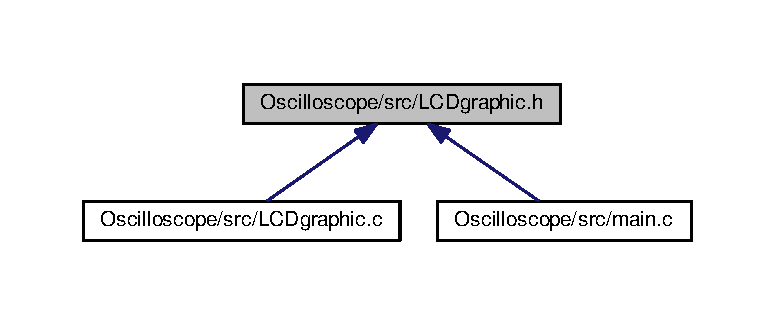
\includegraphics[width=350pt]{LCDgraphic_8h__dep__incl}
\end{center}
\end{figure}
\subsection*{Functions}
\begin{DoxyCompactItemize}
\item 
void \hyperlink{LCDgraphic_8h_a11d5b0d5ef5f8579a4e8d8b078075ec3}{\+\_\+lcd\+\_\+enable} (void)
\begin{DoxyCompactList}\small\item\em Sends the enable pulse. \end{DoxyCompactList}\item 
unsigned char \hyperlink{LCDgraphic_8h_a26ad6217905851ea5c3110a290b6fdb3}{\+\_\+lcd\+\_\+status} (void)
\begin{DoxyCompactList}\small\item\em Reads the status of the L\+C\+D. \end{DoxyCompactList}\item 
void \hyperlink{LCDgraphic_8h_a414751e33fa233791c30874c6737660d}{\+\_\+lcd\+\_\+waitbusy} (void)
\begin{DoxyCompactList}\small\item\em Waits until the L\+C\+D can accept new commands. \end{DoxyCompactList}\item 
void \hyperlink{LCDgraphic_8h_a6d4b16809305b1f89cff88c00862a12e}{L\+C\+Dinit} (void)
\begin{DoxyCompactList}\small\item\em Initializes the L\+C\+D. \end{DoxyCompactList}\item 
void \hyperlink{LCDgraphic_8h_a33c82f86c90f14e8e52f13de0228830d}{L\+C\+Dcmd} (unsigned char data)
\begin{DoxyCompactList}\small\item\em Sends a command to the L\+C\+D. \end{DoxyCompactList}\item 
void \hyperlink{LCDgraphic_8h_a9e0d454df8127abcf7ee2e962b6dd18e}{L\+C\+Dreset} (void)
\begin{DoxyCompactList}\small\item\em Resets the L\+C\+D. \end{DoxyCompactList}\item 
char \hyperlink{LCDgraphic_8h_a84265c7d35e130b40e65accc9196db7f}{L\+C\+Dpage} (unsigned char side, unsigned char page)
\begin{DoxyCompactList}\small\item\em Selects a page from one of the two sides. \end{DoxyCompactList}\item 
void \hyperlink{LCDgraphic_8h_a40db310206fc27ed314f3b955754ee56}{L\+C\+Don} (unsigned char on)
\begin{DoxyCompactList}\small\item\em Turns O\+N/\+O\+F\+F the L\+C\+D. \end{DoxyCompactList}\item 
char \hyperlink{LCDgraphic_8h_a86bbf9d181141b4501339701328da802}{L\+C\+Dchar} (unsigned char c, unsigned char position)
\begin{DoxyCompactList}\small\item\em Writes an A\+S\+C\+I\+I character to the display. \end{DoxyCompactList}\item 
char \hyperlink{LCDgraphic_8h_ac8fd49b1549fc88864cab720cffe7c26}{L\+C\+Dy} (unsigned char side, unsigned char value)
\begin{DoxyCompactList}\small\item\em Specifies a column in the selected page. \end{DoxyCompactList}\item 
void \hyperlink{LCDgraphic_8h_a2efbb5442d0f6110cf5dca2c606e8fff}{L\+C\+Dclear} ()
\begin{DoxyCompactList}\small\item\em Clears all the data in the display. \end{DoxyCompactList}\item 
void \hyperlink{LCDgraphic_8h_a7b3bcf1588c30332104ec4231bbcd959}{emptycolumn} ()
\begin{DoxyCompactList}\small\item\em Writes space between adjacent letters. \end{DoxyCompactList}\item 
void \hyperlink{LCDgraphic_8h_acbbed37c26fb794eb90f33c9a3613649}{xyaxis} ()
\begin{DoxyCompactList}\small\item\em Draws the xy axis grid. \end{DoxyCompactList}\item 
char \hyperlink{LCDgraphic_8h_a1e45984915a2f1966a97fb3bd653bd7d}{lcdplotpixel2} (char rx, char ry, int blank)
\begin{DoxyCompactList}\small\item\em Turns on or off pixels accordingly to blank parameter. \end{DoxyCompactList}\item 
char \hyperlink{LCDgraphic_8h_ae1800a1561ae35e4275a2653532dcb31}{L\+C\+Dstring} (char p, const char $\ast$buffer)
\begin{DoxyCompactList}\small\item\em Writes a string to the L\+C\+D. \end{DoxyCompactList}\item 
char \hyperlink{LCDgraphic_8h_ab9f5dd97e249683eba12ee53b22f2045}{L\+C\+Dstartline} (unsigned char side, unsigned char value)
\begin{DoxyCompactList}\small\item\em Set L\+C\+D start line. \end{DoxyCompactList}\item 
unsigned char \hyperlink{LCDgraphic_8h_a6c9fd9c7e01c9248bd553add98897244}{L\+C\+Dread} ()
\begin{DoxyCompactList}\small\item\em Returns the data written at the previously set page and column. \end{DoxyCompactList}\item 
void \hyperlink{LCDgraphic_8h_ab25dd805ae6efe3ebd124f40d92421ec}{write\+\_\+image} (const char $\ast$image, char top\+\_\+to\+\_\+bottom)
\begin{DoxyCompactList}\small\item\em Writes an image to the screen. \end{DoxyCompactList}\end{DoxyCompactItemize}


\subsection{Detailed Description}
Library with utility functions for graphical L\+C\+D based on K\+S0108. 

\begin{DoxyAuthor}{Author}
Davide Lucchi 
\end{DoxyAuthor}
\begin{DoxyVersion}{Version}
1.\+0 
\end{DoxyVersion}
\begin{DoxySince}{Since}
1.\+0 
\end{DoxySince}


\subsection{Function Documentation}
\hypertarget{LCDgraphic_8h_a11d5b0d5ef5f8579a4e8d8b078075ec3}{}\index{L\+C\+Dgraphic.\+h@{L\+C\+Dgraphic.\+h}!\+\_\+lcd\+\_\+enable@{\+\_\+lcd\+\_\+enable}}
\index{\+\_\+lcd\+\_\+enable@{\+\_\+lcd\+\_\+enable}!L\+C\+Dgraphic.\+h@{L\+C\+Dgraphic.\+h}}
\subsubsection[{\+\_\+lcd\+\_\+enable}]{\setlength{\rightskip}{0pt plus 5cm}void \+\_\+lcd\+\_\+enable (
\begin{DoxyParamCaption}
\item[{void}]{}
\end{DoxyParamCaption}
)}\label{LCDgraphic_8h_a11d5b0d5ef5f8579a4e8d8b078075ec3}


Sends the enable pulse. 

It sends an enable pulse to the L\+C\+D. On the rising edge the L\+C\+D puts/reads the data to/from the bus accordingly to the read/write bit value

\begin{DoxyReturn}{Returns}
nothing
\end{DoxyReturn}
\begin{DoxyAuthor}{Author}
Davide Lucchi 
\end{DoxyAuthor}
\begin{DoxyVersion}{Version}
1.\+0 
\end{DoxyVersion}
\begin{DoxySince}{Since}
1.\+0 
\end{DoxySince}
\hypertarget{LCDgraphic_8h_a26ad6217905851ea5c3110a290b6fdb3}{}\index{L\+C\+Dgraphic.\+h@{L\+C\+Dgraphic.\+h}!\+\_\+lcd\+\_\+status@{\+\_\+lcd\+\_\+status}}
\index{\+\_\+lcd\+\_\+status@{\+\_\+lcd\+\_\+status}!L\+C\+Dgraphic.\+h@{L\+C\+Dgraphic.\+h}}
\subsubsection[{\+\_\+lcd\+\_\+status}]{\setlength{\rightskip}{0pt plus 5cm}unsigned char \+\_\+lcd\+\_\+status (
\begin{DoxyParamCaption}
\item[{void}]{}
\end{DoxyParamCaption}
)}\label{LCDgraphic_8h_a26ad6217905851ea5c3110a290b6fdb3}


Reads the status of the L\+C\+D. 

It sends a request to the L\+C\+D to make it put its status on the data bus. The M\+S\+B of the status contains the B\+U\+S\+Y flag, the 3rd M\+S\+B the display O\+N/\+O\+F\+F flag and the 4th M\+S\+B the R\+E\+S\+E\+T flag.

\begin{DoxyReturn}{Returns}
The L\+C\+D status
\end{DoxyReturn}
\begin{DoxyAuthor}{Author}
Davide Lucchi 
\end{DoxyAuthor}
\begin{DoxyVersion}{Version}
1.\+0 
\end{DoxyVersion}
\begin{DoxySince}{Since}
1.\+0 
\end{DoxySince}
\hypertarget{LCDgraphic_8h_a414751e33fa233791c30874c6737660d}{}\index{L\+C\+Dgraphic.\+h@{L\+C\+Dgraphic.\+h}!\+\_\+lcd\+\_\+waitbusy@{\+\_\+lcd\+\_\+waitbusy}}
\index{\+\_\+lcd\+\_\+waitbusy@{\+\_\+lcd\+\_\+waitbusy}!L\+C\+Dgraphic.\+h@{L\+C\+Dgraphic.\+h}}
\subsubsection[{\+\_\+lcd\+\_\+waitbusy}]{\setlength{\rightskip}{0pt plus 5cm}void \+\_\+lcd\+\_\+waitbusy (
\begin{DoxyParamCaption}
\item[{void}]{}
\end{DoxyParamCaption}
)}\label{LCDgraphic_8h_a414751e33fa233791c30874c6737660d}


Waits until the L\+C\+D can accept new commands. 

It keeps requesting the L\+C\+D status until the B\+U\+S\+Y and R\+E\+S\+E\+T flags are cleared.

\begin{DoxyReturn}{Returns}
nothing
\end{DoxyReturn}
\begin{DoxyAuthor}{Author}
Davide Lucchi 
\end{DoxyAuthor}
\begin{DoxyVersion}{Version}
1.\+0 
\end{DoxyVersion}
\begin{DoxySince}{Since}
1.\+0 
\end{DoxySince}
\hypertarget{LCDgraphic_8h_a7b3bcf1588c30332104ec4231bbcd959}{}\index{L\+C\+Dgraphic.\+h@{L\+C\+Dgraphic.\+h}!emptycolumn@{emptycolumn}}
\index{emptycolumn@{emptycolumn}!L\+C\+Dgraphic.\+h@{L\+C\+Dgraphic.\+h}}
\subsubsection[{emptycolumn}]{\setlength{\rightskip}{0pt plus 5cm}void emptycolumn (
\begin{DoxyParamCaption}
\item[{void}]{}
\end{DoxyParamCaption}
)}\label{LCDgraphic_8h_a7b3bcf1588c30332104ec4231bbcd959}


Writes space between adjacent letters. 

Writes an empty column after the last written letter

\begin{DoxyReturn}{Returns}
nothing
\end{DoxyReturn}
\begin{DoxyAuthor}{Author}
Davide Lucchi 
\end{DoxyAuthor}
\begin{DoxyVersion}{Version}
1.\+0 
\end{DoxyVersion}
\begin{DoxySince}{Since}
1.\+0 
\end{DoxySince}
\hypertarget{LCDgraphic_8h_a86bbf9d181141b4501339701328da802}{}\index{L\+C\+Dgraphic.\+h@{L\+C\+Dgraphic.\+h}!L\+C\+Dchar@{L\+C\+Dchar}}
\index{L\+C\+Dchar@{L\+C\+Dchar}!L\+C\+Dgraphic.\+h@{L\+C\+Dgraphic.\+h}}
\subsubsection[{L\+C\+Dchar}]{\setlength{\rightskip}{0pt plus 5cm}char L\+C\+Dchar (
\begin{DoxyParamCaption}
\item[{unsigned char}]{c, }
\item[{unsigned char}]{position}
\end{DoxyParamCaption}
)}\label{LCDgraphic_8h_a86bbf9d181141b4501339701328da802}


Writes an A\+S\+C\+I\+I character to the display. 

Writes an A\+S\+C\+I\+I character to the formerly specified position with \hyperlink{LCDgraphic_8c_a84265c7d35e130b40e65accc9196db7f}{L\+C\+Dpage()} and \hyperlink{LCDgraphic_8c_ac8fd49b1549fc88864cab720cffe7c26}{L\+C\+Dy()} or to the position specified by the position parameter


\begin{DoxyParams}{Parameters}
{\em c} & The character to write \\
\hline
{\em position} & {\ttfamily 0} use formerly specified position; {\ttfamily 1} left; {\ttfamily 2} center; {\ttfamily 3} right. \\
\hline
\end{DoxyParams}
\begin{DoxyReturn}{Returns}
{\ttfamily 0} if success {\ttfamily -\/1} if it fails
\end{DoxyReturn}
\begin{DoxyAuthor}{Author}
Davide Lucchi 
\end{DoxyAuthor}
\begin{DoxyVersion}{Version}
1.\+0 
\end{DoxyVersion}
\begin{DoxySince}{Since}
1.\+0
\end{DoxySince}
Writes an A\+S\+C\+I\+I character to the formerly specified position with \hyperlink{LCDgraphic_8c_a84265c7d35e130b40e65accc9196db7f}{L\+C\+Dpage()} and \hyperlink{LCDgraphic_8c_ac8fd49b1549fc88864cab720cffe7c26}{L\+C\+Dy()} or to the position specified by the position parameter


\begin{DoxyParams}{Parameters}
{\em c} & the character to write \\
\hline
{\em position} & {\ttfamily 0} use formerly specified position; {\ttfamily 1} left; {\ttfamily 2} center; {\ttfamily 3} right. \\
\hline
\end{DoxyParams}
\begin{DoxyReturn}{Returns}
{\ttfamily 0} if success, {\ttfamily -\/1} if fail
\end{DoxyReturn}
\begin{DoxyAuthor}{Author}
Davide Lucchi 
\end{DoxyAuthor}
\begin{DoxyVersion}{Version}
1.\+0 
\end{DoxyVersion}
\begin{DoxySince}{Since}
1.\+0 
\end{DoxySince}
\hypertarget{LCDgraphic_8h_a2efbb5442d0f6110cf5dca2c606e8fff}{}\index{L\+C\+Dgraphic.\+h@{L\+C\+Dgraphic.\+h}!L\+C\+Dclear@{L\+C\+Dclear}}
\index{L\+C\+Dclear@{L\+C\+Dclear}!L\+C\+Dgraphic.\+h@{L\+C\+Dgraphic.\+h}}
\subsubsection[{L\+C\+Dclear}]{\setlength{\rightskip}{0pt plus 5cm}void L\+C\+Dclear (
\begin{DoxyParamCaption}
\item[{void}]{}
\end{DoxyParamCaption}
)}\label{LCDgraphic_8h_a2efbb5442d0f6110cf5dca2c606e8fff}


Clears all the data in the display. 

\begin{DoxyReturn}{Returns}
nothing
\end{DoxyReturn}
\begin{DoxyAuthor}{Author}
Davide Lucchi 
\end{DoxyAuthor}
\begin{DoxyVersion}{Version}
1.\+0 
\end{DoxyVersion}
\begin{DoxySince}{Since}
1.\+0 
\end{DoxySince}
\hypertarget{LCDgraphic_8h_a33c82f86c90f14e8e52f13de0228830d}{}\index{L\+C\+Dgraphic.\+h@{L\+C\+Dgraphic.\+h}!L\+C\+Dcmd@{L\+C\+Dcmd}}
\index{L\+C\+Dcmd@{L\+C\+Dcmd}!L\+C\+Dgraphic.\+h@{L\+C\+Dgraphic.\+h}}
\subsubsection[{L\+C\+Dcmd}]{\setlength{\rightskip}{0pt plus 5cm}void L\+C\+Dcmd (
\begin{DoxyParamCaption}
\item[{unsigned char}]{data}
\end{DoxyParamCaption}
)}\label{LCDgraphic_8h_a33c82f86c90f14e8e52f13de0228830d}


Sends a command to the L\+C\+D. 

It writes an 8bits value on the data bus and sends an enable pulse to make the L\+C\+D read the value.


\begin{DoxyParams}{Parameters}
{\em data} & the 8bits value to send to the L\+C\+D \\
\hline
\end{DoxyParams}
\begin{DoxyReturn}{Returns}
nothing
\end{DoxyReturn}
\begin{DoxyAuthor}{Author}
Davide Lucchi 
\end{DoxyAuthor}
\begin{DoxyVersion}{Version}
1.\+0 
\end{DoxyVersion}
\begin{DoxySince}{Since}
1.\+0 
\end{DoxySince}
\hypertarget{LCDgraphic_8h_a6d4b16809305b1f89cff88c00862a12e}{}\index{L\+C\+Dgraphic.\+h@{L\+C\+Dgraphic.\+h}!L\+C\+Dinit@{L\+C\+Dinit}}
\index{L\+C\+Dinit@{L\+C\+Dinit}!L\+C\+Dgraphic.\+h@{L\+C\+Dgraphic.\+h}}
\subsubsection[{L\+C\+Dinit}]{\setlength{\rightskip}{0pt plus 5cm}void L\+C\+Dinit (
\begin{DoxyParamCaption}
\item[{void}]{}
\end{DoxyParamCaption}
)}\label{LCDgraphic_8h_a6d4b16809305b1f89cff88c00862a12e}


Initializes the L\+C\+D. 

Waits until L\+C\+D is no longer busy, then sends reset signal and turns L\+C\+D O\+N.

\begin{DoxyReturn}{Returns}
nothing
\end{DoxyReturn}
\begin{DoxyAuthor}{Author}
Davide Lucchi 
\end{DoxyAuthor}
\begin{DoxyVersion}{Version}
1.\+0 
\end{DoxyVersion}
\begin{DoxySince}{Since}
1.\+0 
\end{DoxySince}
\hypertarget{LCDgraphic_8h_a40db310206fc27ed314f3b955754ee56}{}\index{L\+C\+Dgraphic.\+h@{L\+C\+Dgraphic.\+h}!L\+C\+Don@{L\+C\+Don}}
\index{L\+C\+Don@{L\+C\+Don}!L\+C\+Dgraphic.\+h@{L\+C\+Dgraphic.\+h}}
\subsubsection[{L\+C\+Don}]{\setlength{\rightskip}{0pt plus 5cm}void L\+C\+Don (
\begin{DoxyParamCaption}
\item[{unsigned char}]{on}
\end{DoxyParamCaption}
)}\label{LCDgraphic_8h_a40db310206fc27ed314f3b955754ee56}


Turns O\+N/\+O\+F\+F the L\+C\+D. 


\begin{DoxyParams}{Parameters}
{\em on} & {\ttfamily 1} O\+N; {\ttfamily 0} O\+F\+F \\
\hline
\end{DoxyParams}
\begin{DoxyReturn}{Returns}
nothing
\end{DoxyReturn}
\begin{DoxyAuthor}{Author}
Davide Lucchi 
\end{DoxyAuthor}
\begin{DoxyVersion}{Version}
1.\+0 
\end{DoxyVersion}
\begin{DoxySince}{Since}
1.\+0 
\end{DoxySince}
\hypertarget{LCDgraphic_8h_a84265c7d35e130b40e65accc9196db7f}{}\index{L\+C\+Dgraphic.\+h@{L\+C\+Dgraphic.\+h}!L\+C\+Dpage@{L\+C\+Dpage}}
\index{L\+C\+Dpage@{L\+C\+Dpage}!L\+C\+Dgraphic.\+h@{L\+C\+Dgraphic.\+h}}
\subsubsection[{L\+C\+Dpage}]{\setlength{\rightskip}{0pt plus 5cm}char L\+C\+Dpage (
\begin{DoxyParamCaption}
\item[{unsigned char}]{side, }
\item[{unsigned char}]{page}
\end{DoxyParamCaption}
)}\label{LCDgraphic_8h_a84265c7d35e130b40e65accc9196db7f}


Selects a page from one of the two sides. 

The L\+C\+D screen is divided into two sides each consisting of 64x64 pixels. Each side is horizontally divided in 8 pages each 8 pixels high.


\begin{DoxyParams}{Parameters}
{\em side} & Selects the side. {\ttfamily 0} for left side, {\ttfamily 1} for right side and {\ttfamily 2} for both sides. \\
\hline
{\em page} & Selects one of the {\ttfamily 8} pages. Accepts values from {\ttfamily 0} to {\ttfamily 7} \\
\hline
\end{DoxyParams}
\begin{DoxyReturn}{Returns}
{\ttfamily 0} if success {\ttfamily -\/1} if it fails
\end{DoxyReturn}
\begin{DoxyAuthor}{Author}
Davide Lucchi 
\end{DoxyAuthor}
\begin{DoxyVersion}{Version}
1.\+0 
\end{DoxyVersion}
\begin{DoxySince}{Since}
1.\+0
\end{DoxySince}
The L\+C\+D screen is divided into two pages each consisting of 64x64 pixels. Each page is horizontally divided in 8 rows each 8 pixels high.


\begin{DoxyParams}{Parameters}
{\em side} & Selects the side. 0 for left side, 1 for right side and 2 for both sides. \\
\hline
{\em page} & Selects one of the 8 pages. Accepts values from {\ttfamily 0} to {\ttfamily 7} \\
\hline
\end{DoxyParams}
\begin{DoxyReturn}{Returns}
{\ttfamily 0} if success {\ttfamily -\/1} if it fails
\end{DoxyReturn}
\begin{DoxyAuthor}{Author}
Davide Lucchi 
\end{DoxyAuthor}
\begin{DoxyVersion}{Version}
1.\+0 
\end{DoxyVersion}
\begin{DoxySince}{Since}
1.\+0 
\end{DoxySince}
\hypertarget{LCDgraphic_8h_a1e45984915a2f1966a97fb3bd653bd7d}{}\index{L\+C\+Dgraphic.\+h@{L\+C\+Dgraphic.\+h}!lcdplotpixel2@{lcdplotpixel2}}
\index{lcdplotpixel2@{lcdplotpixel2}!L\+C\+Dgraphic.\+h@{L\+C\+Dgraphic.\+h}}
\subsubsection[{lcdplotpixel2}]{\setlength{\rightskip}{0pt plus 5cm}char lcdplotpixel2 (
\begin{DoxyParamCaption}
\item[{char}]{rx, }
\item[{char}]{ry, }
\item[{int}]{blank}
\end{DoxyParamCaption}
)}\label{LCDgraphic_8h_a1e45984915a2f1966a97fb3bd653bd7d}


Turns on or off pixels accordingly to blank parameter. 


\begin{DoxyParams}{Parameters}
{\em rx} & x coordinate \\
\hline
{\em ry} & y coordinate \\
\hline
{\em blank} & {\ttfamily -\/1} turns off all pixels of the column {\ttfamily 0} turns on specified pixel {\ttfamily 1} turns off only specified pixel \\
\hline
\end{DoxyParams}
\begin{DoxyReturn}{Returns}
{\ttfamily 0} if success {\ttfamily -\/1} if it fails
\end{DoxyReturn}
\begin{DoxyAuthor}{Author}
Davide Lucchi 
\end{DoxyAuthor}
\begin{DoxyVersion}{Version}
1.\+0 
\end{DoxyVersion}
\begin{DoxySince}{Since}
1.\+0 
\end{DoxySince}
\hypertarget{LCDgraphic_8h_a6c9fd9c7e01c9248bd553add98897244}{}\index{L\+C\+Dgraphic.\+h@{L\+C\+Dgraphic.\+h}!L\+C\+Dread@{L\+C\+Dread}}
\index{L\+C\+Dread@{L\+C\+Dread}!L\+C\+Dgraphic.\+h@{L\+C\+Dgraphic.\+h}}
\subsubsection[{L\+C\+Dread}]{\setlength{\rightskip}{0pt plus 5cm}unsigned char L\+C\+Dread (
\begin{DoxyParamCaption}
{}
\end{DoxyParamCaption}
)}\label{LCDgraphic_8h_a6c9fd9c7e01c9248bd553add98897244}


Returns the data written at the previously set page and column. 

\begin{DoxyReturn}{Returns}
Returns the data written at the previously set page and column
\end{DoxyReturn}
\begin{DoxyAuthor}{Author}
Davide Lucchi 
\end{DoxyAuthor}
\begin{DoxyVersion}{Version}
1.\+0 
\end{DoxyVersion}
\begin{DoxySince}{Since}
1.\+0 
\end{DoxySince}
\hypertarget{LCDgraphic_8h_a9e0d454df8127abcf7ee2e962b6dd18e}{}\index{L\+C\+Dgraphic.\+h@{L\+C\+Dgraphic.\+h}!L\+C\+Dreset@{L\+C\+Dreset}}
\index{L\+C\+Dreset@{L\+C\+Dreset}!L\+C\+Dgraphic.\+h@{L\+C\+Dgraphic.\+h}}
\subsubsection[{L\+C\+Dreset}]{\setlength{\rightskip}{0pt plus 5cm}void L\+C\+Dreset (
\begin{DoxyParamCaption}
\item[{void}]{}
\end{DoxyParamCaption}
)}\label{LCDgraphic_8h_a9e0d454df8127abcf7ee2e962b6dd18e}


Resets the L\+C\+D. 

It sends a zero pulse to the L\+C\+D to make it reset and waits until L\+C\+D B\+U\+S\+Y and R\+E\+S\+E\+T\+S flags are cleared.

\begin{DoxyReturn}{Returns}
nothing
\end{DoxyReturn}
\begin{DoxyAuthor}{Author}
Davide Lucchi 
\end{DoxyAuthor}
\begin{DoxyVersion}{Version}
1.\+0 
\end{DoxyVersion}
\begin{DoxySince}{Since}
1.\+0 
\end{DoxySince}
\hypertarget{LCDgraphic_8h_ab9f5dd97e249683eba12ee53b22f2045}{}\index{L\+C\+Dgraphic.\+h@{L\+C\+Dgraphic.\+h}!L\+C\+Dstartline@{L\+C\+Dstartline}}
\index{L\+C\+Dstartline@{L\+C\+Dstartline}!L\+C\+Dgraphic.\+h@{L\+C\+Dgraphic.\+h}}
\subsubsection[{L\+C\+Dstartline}]{\setlength{\rightskip}{0pt plus 5cm}char L\+C\+Dstartline (
\begin{DoxyParamCaption}
\item[{unsigned char}]{side, }
\item[{unsigned char}]{value}
\end{DoxyParamCaption}
)}\label{LCDgraphic_8h_ab9f5dd97e249683eba12ee53b22f2045}


Set L\+C\+D start line. 


\begin{DoxyParams}{Parameters}
{\em side} & Selects the side. {\ttfamily 0} for left side, {\ttfamily 1} for right side and {\ttfamily 2} for both sides. \\
\hline
{\em value} & The display start line value between {\ttfamily 0} and {\ttfamily 64} \\
\hline
\end{DoxyParams}
\begin{DoxyReturn}{Returns}
{\ttfamily 0} if success {\ttfamily -\/1} if it fails
\end{DoxyReturn}
\begin{DoxyAuthor}{Author}
Davide Lucchi 
\end{DoxyAuthor}
\begin{DoxyVersion}{Version}
1.\+0 
\end{DoxyVersion}
\begin{DoxySince}{Since}
1.\+0 
\end{DoxySince}
\hypertarget{LCDgraphic_8h_ae1800a1561ae35e4275a2653532dcb31}{}\index{L\+C\+Dgraphic.\+h@{L\+C\+Dgraphic.\+h}!L\+C\+Dstring@{L\+C\+Dstring}}
\index{L\+C\+Dstring@{L\+C\+Dstring}!L\+C\+Dgraphic.\+h@{L\+C\+Dgraphic.\+h}}
\subsubsection[{L\+C\+Dstring}]{\setlength{\rightskip}{0pt plus 5cm}char L\+C\+Dstring (
\begin{DoxyParamCaption}
\item[{char}]{p, }
\item[{const char $\ast$}]{buffer}
\end{DoxyParamCaption}
)}\label{LCDgraphic_8h_ae1800a1561ae35e4275a2653532dcb31}


Writes a string to the L\+C\+D. 

Writes the string at the formerly specified position or at the {\ttfamily p} defined position


\begin{DoxyParams}{Parameters}
{\em p} & {\ttfamily 0} formerly specified position; {\ttfamily 1} left aligned; {\ttfamily 2} centered; {\ttfamily 3} right aligned \\
\hline
{\em buffer} & The string to print \\
\hline
\end{DoxyParams}
\begin{DoxyReturn}{Returns}
{\ttfamily 0} if success {\ttfamily -\/1} if it fails
\end{DoxyReturn}
\begin{DoxyAuthor}{Author}
Davide Lucchi 
\end{DoxyAuthor}
\begin{DoxyVersion}{Version}
1.\+0 
\end{DoxyVersion}
\begin{DoxySince}{Since}
1.\+0
\end{DoxySince}
Writes the string at the formerly specified position or at the {\ttfamily p} defined position


\begin{DoxyParams}{Parameters}
{\em p} & {\ttfamily 0} formerly specified position; {\ttfamily 1} left aligned; {\ttfamily 2} centered; {\ttfamily 3} right aligned \\
\hline
{\em buffer} & the string to print \\
\hline
\end{DoxyParams}
\begin{DoxyReturn}{Returns}
{\ttfamily 0} if success, {\ttfamily -\/1} if fail
\end{DoxyReturn}
\begin{DoxyAuthor}{Author}
Davide Lucchi 
\end{DoxyAuthor}
\begin{DoxyVersion}{Version}
1.\+0 
\end{DoxyVersion}
\begin{DoxySince}{Since}
1.\+0 
\end{DoxySince}
\hypertarget{LCDgraphic_8h_ac8fd49b1549fc88864cab720cffe7c26}{}\index{L\+C\+Dgraphic.\+h@{L\+C\+Dgraphic.\+h}!L\+C\+Dy@{L\+C\+Dy}}
\index{L\+C\+Dy@{L\+C\+Dy}!L\+C\+Dgraphic.\+h@{L\+C\+Dgraphic.\+h}}
\subsubsection[{L\+C\+Dy}]{\setlength{\rightskip}{0pt plus 5cm}char L\+C\+Dy (
\begin{DoxyParamCaption}
\item[{unsigned char}]{side, }
\item[{unsigned char}]{value}
\end{DoxyParamCaption}
)}\label{LCDgraphic_8h_ac8fd49b1549fc88864cab720cffe7c26}


Specifies a column in the selected page. 

Each page contains 64 columns of 8 pixels each. It selects one of these columns.


\begin{DoxyParams}{Parameters}
{\em side} & Selects the side. {\ttfamily 0} for left side, {\ttfamily 1} for right side and {\ttfamily 2} for both sides. \\
\hline
{\em value} & The column value between {\ttfamily 0} and {\ttfamily 63} \\
\hline
\end{DoxyParams}
\begin{DoxyReturn}{Returns}
{\ttfamily 0} if success {\ttfamily -\/1} if it fails
\end{DoxyReturn}
\begin{DoxyAuthor}{Author}
Davide Lucchi 
\end{DoxyAuthor}
\begin{DoxyVersion}{Version}
1.\+0 
\end{DoxyVersion}
\begin{DoxySince}{Since}
1.\+0 
\end{DoxySince}
\hypertarget{LCDgraphic_8h_ab25dd805ae6efe3ebd124f40d92421ec}{}\index{L\+C\+Dgraphic.\+h@{L\+C\+Dgraphic.\+h}!write\+\_\+image@{write\+\_\+image}}
\index{write\+\_\+image@{write\+\_\+image}!L\+C\+Dgraphic.\+h@{L\+C\+Dgraphic.\+h}}
\subsubsection[{write\+\_\+image}]{\setlength{\rightskip}{0pt plus 5cm}void write\+\_\+image (
\begin{DoxyParamCaption}
\item[{const char $\ast$}]{image, }
\item[{char}]{top\+\_\+to\+\_\+bottom}
\end{DoxyParamCaption}
)}\label{LCDgraphic_8h_ab25dd805ae6efe3ebd124f40d92421ec}


Writes an image to the screen. 

It writes the image passed as argument to the screen. The argument must meet certain requirements. It must contain 128$\ast$8 8bit values, one for each column of each page of the display. The array is written to the L\+C\+D from left to right starting at page 0 end ending at page 7.


\begin{DoxyParams}{Parameters}
{\em image} & An array with the image to write \\
\hline
{\em top\+\_\+to\+\_\+bottom} & {\ttfamily 0} if the M\+S\+B of the 8 bit values is the top pixel, {\ttfamily 1} otherwise \\
\hline
\end{DoxyParams}
\begin{DoxyReturn}{Returns}
nothing
\end{DoxyReturn}
\begin{DoxyAuthor}{Author}
Davide Lucchi 
\end{DoxyAuthor}
\begin{DoxyVersion}{Version}
1.\+0 
\end{DoxyVersion}
\begin{DoxySince}{Since}
1.\+0 
\end{DoxySince}
\hypertarget{LCDgraphic_8h_acbbed37c26fb794eb90f33c9a3613649}{}\index{L\+C\+Dgraphic.\+h@{L\+C\+Dgraphic.\+h}!xyaxis@{xyaxis}}
\index{xyaxis@{xyaxis}!L\+C\+Dgraphic.\+h@{L\+C\+Dgraphic.\+h}}
\subsubsection[{xyaxis}]{\setlength{\rightskip}{0pt plus 5cm}void xyaxis (
\begin{DoxyParamCaption}
{}
\end{DoxyParamCaption}
)}\label{LCDgraphic_8h_acbbed37c26fb794eb90f33c9a3613649}


Draws the xy axis grid. 

\begin{DoxyReturn}{Returns}
nothing
\end{DoxyReturn}
\begin{DoxyAuthor}{Author}
Davide Lucchi 
\end{DoxyAuthor}
\begin{DoxyVersion}{Version}
1.\+0 
\end{DoxyVersion}
\begin{DoxySince}{Since}
1.\+0 
\end{DoxySince}

\hypertarget{main_8c}{}\section{Oscilloscope/src/main.c File Reference}
\label{main_8c}\index{Oscilloscope/src/main.\+c@{Oscilloscope/src/main.\+c}}


Oscilloscope based on P\+I\+C18\+F4550 and 128x64 Graphic L\+C\+D.  


{\ttfamily \#include $<$xc.\+h$>$}\\*
{\ttfamily \#include $<$p18f4550.\+h$>$}\\*
{\ttfamily \#include $<$string.\+h$>$}\\*
{\ttfamily \#include \char`\"{}L\+C\+Dgraphic.\+h\char`\"{}}\\*
{\ttfamily \#include $<$stdio.\+h$>$}\\*
Include dependency graph for main.\+c\+:\nopagebreak
\begin{figure}[H]
\begin{center}
\leavevmode
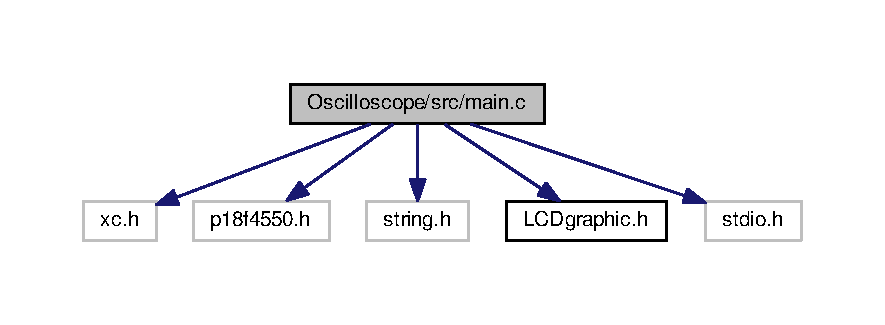
\includegraphics[width=350pt]{main_8c__incl}
\end{center}
\end{figure}
\subsection*{Macros}
\begin{DoxyCompactItemize}
\item 
\hypertarget{main_8c_a024148e99a7143db044a48216664d03d}{}\#define {\bfseries \+\_\+\+X\+T\+A\+L\+\_\+\+F\+R\+E\+Q}~40000000\label{main_8c_a024148e99a7143db044a48216664d03d}

\item 
\hypertarget{main_8c_a8ef631897418d17fbf93f4845d384269}{}\#define {\bfseries S\+C\+R\+E\+E\+N\+\_\+\+F\+R\+E\+E\+Z\+E}~P\+O\+R\+T\+Bbits.\+R\+B0\label{main_8c_a8ef631897418d17fbf93f4845d384269}

\item 
\hypertarget{main_8c_a05e4c020b74c9964cf41e8eb06bd3d47}{}\#define {\bfseries H\+\_\+\+V}~P\+O\+R\+T\+Bbits.\+R\+B1\label{main_8c_a05e4c020b74c9964cf41e8eb06bd3d47}

\end{DoxyCompactItemize}
\subsection*{Functions}
\begin{DoxyCompactItemize}
\item 
\hypertarget{main_8c_aa80441bd92270f050b0796561243f410}{}int {\bfseries abs} (int a)\label{main_8c_aa80441bd92270f050b0796561243f410}

\item 
void \hyperlink{main_8c_a6288eba0f8e8ad3ab1544ad731eb7667}{main} (void)
\begin{DoxyCompactList}\small\item\em Oscilloscope based on P\+I\+C18\+F4550 and 128x64 Graphic L\+C\+D. \end{DoxyCompactList}\end{DoxyCompactItemize}
\subsection*{Variables}
\begin{DoxyCompactItemize}
\item 
\hypertarget{main_8c_a1bf5468b2b2a6cb7878b046d50a4f95e}{}char const {\bfseries image} \mbox{[}$\,$\mbox{]}\label{main_8c_a1bf5468b2b2a6cb7878b046d50a4f95e}

\end{DoxyCompactItemize}


\subsection{Detailed Description}
Oscilloscope based on P\+I\+C18\+F4550 and 128x64 Graphic L\+C\+D. 

\begin{DoxyAuthor}{Author}
Davide Lucchi 
\end{DoxyAuthor}
\begin{DoxyVersion}{Version}
1.\+0 
\end{DoxyVersion}
\begin{DoxySince}{Since}
1.\+0 
\end{DoxySince}


\subsection{Function Documentation}
\hypertarget{main_8c_a6288eba0f8e8ad3ab1544ad731eb7667}{}\index{main.\+c@{main.\+c}!main@{main}}
\index{main@{main}!main.\+c@{main.\+c}}
\subsubsection[{main}]{\setlength{\rightskip}{0pt plus 5cm}void main (
\begin{DoxyParamCaption}
\item[{void}]{}
\end{DoxyParamCaption}
)}\label{main_8c_a6288eba0f8e8ad3ab1544ad731eb7667}


Oscilloscope based on P\+I\+C18\+F4550 and 128x64 Graphic L\+C\+D. 

\begin{DoxyReturn}{Returns}
nothing
\end{DoxyReturn}
\begin{DoxyAuthor}{Author}
Davide Lucchi 
\end{DoxyAuthor}
\begin{DoxyVersion}{Version}
1.\+0 
\end{DoxyVersion}
\begin{DoxySince}{Since}
1.\+0 
\end{DoxySince}

%--- End generated contents ---

% Index
\backmatter
\newpage
\phantomsection
\clearemptydoublepage
\addcontentsline{toc}{chapter}{Index}
\printindex

\end{document}
